\documentclass[12pt,]{article}
\usepackage{lmodern}
\usepackage{amssymb,amsmath}
\usepackage{ifxetex,ifluatex}
\usepackage{fixltx2e} % provides \textsubscript
\ifnum 0\ifxetex 1\fi\ifluatex 1\fi=0 % if pdftex
  \usepackage[T1]{fontenc}
  \usepackage[utf8]{inputenc}
\else % if luatex or xelatex
  \ifxetex
    \usepackage{mathspec}
  \else
    \usepackage{fontspec}
  \fi
  \defaultfontfeatures{Ligatures=TeX,Scale=MatchLowercase}
\fi
% use upquote if available, for straight quotes in verbatim environments
\IfFileExists{upquote.sty}{\usepackage{upquote}}{}
% use microtype if available
\IfFileExists{microtype.sty}{%
\usepackage{microtype}
\UseMicrotypeSet[protrusion]{basicmath} % disable protrusion for tt fonts
}{}
\usepackage[margin=1in]{geometry}
\usepackage{hyperref}
\hypersetup{unicode=true,
            pdftitle={Homework 1},
            pdfauthor={Emily Robinson},
            pdfborder={0 0 0},
            breaklinks=true}
\urlstyle{same}  % don't use monospace font for urls
\usepackage{color}
\usepackage{fancyvrb}
\newcommand{\VerbBar}{|}
\newcommand{\VERB}{\Verb[commandchars=\\\{\}]}
\DefineVerbatimEnvironment{Highlighting}{Verbatim}{commandchars=\\\{\}}
% Add ',fontsize=\small' for more characters per line
\usepackage{framed}
\definecolor{shadecolor}{RGB}{248,248,248}
\newenvironment{Shaded}{\begin{snugshade}}{\end{snugshade}}
\newcommand{\AlertTok}[1]{\textcolor[rgb]{0.94,0.16,0.16}{#1}}
\newcommand{\AnnotationTok}[1]{\textcolor[rgb]{0.56,0.35,0.01}{\textbf{\textit{#1}}}}
\newcommand{\AttributeTok}[1]{\textcolor[rgb]{0.77,0.63,0.00}{#1}}
\newcommand{\BaseNTok}[1]{\textcolor[rgb]{0.00,0.00,0.81}{#1}}
\newcommand{\BuiltInTok}[1]{#1}
\newcommand{\CharTok}[1]{\textcolor[rgb]{0.31,0.60,0.02}{#1}}
\newcommand{\CommentTok}[1]{\textcolor[rgb]{0.56,0.35,0.01}{\textit{#1}}}
\newcommand{\CommentVarTok}[1]{\textcolor[rgb]{0.56,0.35,0.01}{\textbf{\textit{#1}}}}
\newcommand{\ConstantTok}[1]{\textcolor[rgb]{0.00,0.00,0.00}{#1}}
\newcommand{\ControlFlowTok}[1]{\textcolor[rgb]{0.13,0.29,0.53}{\textbf{#1}}}
\newcommand{\DataTypeTok}[1]{\textcolor[rgb]{0.13,0.29,0.53}{#1}}
\newcommand{\DecValTok}[1]{\textcolor[rgb]{0.00,0.00,0.81}{#1}}
\newcommand{\DocumentationTok}[1]{\textcolor[rgb]{0.56,0.35,0.01}{\textbf{\textit{#1}}}}
\newcommand{\ErrorTok}[1]{\textcolor[rgb]{0.64,0.00,0.00}{\textbf{#1}}}
\newcommand{\ExtensionTok}[1]{#1}
\newcommand{\FloatTok}[1]{\textcolor[rgb]{0.00,0.00,0.81}{#1}}
\newcommand{\FunctionTok}[1]{\textcolor[rgb]{0.00,0.00,0.00}{#1}}
\newcommand{\ImportTok}[1]{#1}
\newcommand{\InformationTok}[1]{\textcolor[rgb]{0.56,0.35,0.01}{\textbf{\textit{#1}}}}
\newcommand{\KeywordTok}[1]{\textcolor[rgb]{0.13,0.29,0.53}{\textbf{#1}}}
\newcommand{\NormalTok}[1]{#1}
\newcommand{\OperatorTok}[1]{\textcolor[rgb]{0.81,0.36,0.00}{\textbf{#1}}}
\newcommand{\OtherTok}[1]{\textcolor[rgb]{0.56,0.35,0.01}{#1}}
\newcommand{\PreprocessorTok}[1]{\textcolor[rgb]{0.56,0.35,0.01}{\textit{#1}}}
\newcommand{\RegionMarkerTok}[1]{#1}
\newcommand{\SpecialCharTok}[1]{\textcolor[rgb]{0.00,0.00,0.00}{#1}}
\newcommand{\SpecialStringTok}[1]{\textcolor[rgb]{0.31,0.60,0.02}{#1}}
\newcommand{\StringTok}[1]{\textcolor[rgb]{0.31,0.60,0.02}{#1}}
\newcommand{\VariableTok}[1]{\textcolor[rgb]{0.00,0.00,0.00}{#1}}
\newcommand{\VerbatimStringTok}[1]{\textcolor[rgb]{0.31,0.60,0.02}{#1}}
\newcommand{\WarningTok}[1]{\textcolor[rgb]{0.56,0.35,0.01}{\textbf{\textit{#1}}}}
\usepackage{longtable,booktabs}
\usepackage{graphicx,grffile}
\makeatletter
\def\maxwidth{\ifdim\Gin@nat@width>\linewidth\linewidth\else\Gin@nat@width\fi}
\def\maxheight{\ifdim\Gin@nat@height>\textheight\textheight\else\Gin@nat@height\fi}
\makeatother
% Scale images if necessary, so that they will not overflow the page
% margins by default, and it is still possible to overwrite the defaults
% using explicit options in \includegraphics[width, height, ...]{}
\setkeys{Gin}{width=\maxwidth,height=\maxheight,keepaspectratio}
\IfFileExists{parskip.sty}{%
\usepackage{parskip}
}{% else
\setlength{\parindent}{0pt}
\setlength{\parskip}{6pt plus 2pt minus 1pt}
}
\setlength{\emergencystretch}{3em}  % prevent overfull lines
\providecommand{\tightlist}{%
  \setlength{\itemsep}{0pt}\setlength{\parskip}{0pt}}
\setcounter{secnumdepth}{0}
% Redefines (sub)paragraphs to behave more like sections
\ifx\paragraph\undefined\else
\let\oldparagraph\paragraph
\renewcommand{\paragraph}[1]{\oldparagraph{#1}\mbox{}}
\fi
\ifx\subparagraph\undefined\else
\let\oldsubparagraph\subparagraph
\renewcommand{\subparagraph}[1]{\oldsubparagraph{#1}\mbox{}}
\fi

%%% Use protect on footnotes to avoid problems with footnotes in titles
\let\rmarkdownfootnote\footnote%
\def\footnote{\protect\rmarkdownfootnote}

%%% Change title format to be more compact
\usepackage{titling}

% Create subtitle command for use in maketitle
\providecommand{\subtitle}[1]{
  \posttitle{
    \begin{center}\large#1\end{center}
    }
}

\setlength{\droptitle}{-2em}

  \title{Homework 1}
    \pretitle{\vspace{\droptitle}\centering\huge}
  \posttitle{\par}
  \subtitle{STAT 984}
  \author{Emily Robinson}
    \preauthor{\centering\large\emph}
  \postauthor{\par}
      \predate{\centering\large\emph}
  \postdate{\par}
    \date{September 5, 2019}

\usepackage{amsmath}
\usepackage{amssymb}
\usepackage{amsthm}

\begin{document}
\maketitle

\hypertarget{exercise-1.1}{%
\subsubsection{Exercise 1.1}\label{exercise-1.1}}

Assume that \(a_n \rightarrow a\) and \(b_n \rightarrow b\), where \(a\)
and \(b\) are real numbers.

\begin{enumerate}
\def\labelenumi{\alph{enumi}.}
\tightlist
\item
  Prove that \(a_nb_n \rightarrow ab\).
\end{enumerate}

\begin{proof}
Let $a_n$ and $b_n$ be sequences and suppose $a_n \rightarrow a$ and $b_n \rightarrow b$ for real numbers $a$ and $b$. Then $\{a_n\}_{n\ge1}$ and $\{b_n\}_{n\ge1}$ are bounded.Thus, there exists an $M>0$ such that $|a_n|\le M$ for all $n\ge 1$. Consider two cases: $b=0$ and $b\ne 0$.

Case 1: Let $b = 0$. By definition of convergence (Definition 1.1), there exists some $N_1>0$ such that for all $n\ge N_1$, $|b_n-b|<\frac{\epsilon}{M}.$ Then
\begin{align*}
|a_nb_n-ab| & = |a_nb_n-a_nb+a_b-ab|\\
& = |a_n(b_n-b)+b(a_n-a)|\\
& \le |a_n(b_n-b)| +|b(a_n-a)|\\
& =|a_n||b_n-b|+|b||a_n-a|\\
& < M\left(\frac{\epsilon}{M}\right)+0\\
& = \epsilon.
\end{align*}
Case 2: Let $b \ne 0$. Then there exists $N_2>0$ such that for all $n\ge N_2$, $|b_n-b|<\frac{\epsilon}{2M}$ and there exists $N_3>0$ such that for all $n \ge N_3$, $|a_n-a|<\frac{\epsilon}{2|b|}$. Then
\begin{align*}
|a_nb_n-ab| & = |a_nb_n-a_nb+a_b-ab|\\
& = |a_n(b_n-b)+b(a_n-a)|\\
& \le |a_n(b_n-b)| +|b(a_n-a)|\\
& =|a_n||b_n-b|+|b||a_n-a|\\
& < M\left(\frac{\epsilon}{2M}\right)+|b|\left(\frac{\epsilon}{2|b|}\right)\\
& = \epsilon.
\end{align*}
Therefore, for all $\epsilon>0$, there exists $N = max\{N_1, N_2, N_3\}$, such that for all $n\ge N,$ $|a_nb_n-ab|<\epsilon.$ Thus, $a_nb_n\rightarrow ab.$
\end{proof}

\newpage

\begin{enumerate}
\def\labelenumi{\alph{enumi}.}
\setcounter{enumi}{1}
\tightlist
\item
  Prove that if \(b \ne 0\), \(a_n/b_n \rightarrow a/b.\)
\end{enumerate}

\begin{proof}
Let $a_n$ and $b_n$ be sequences and suppose $a_n \rightarrow a$ and $b_n \rightarrow b$ for $b\ne 0.$ Let $\epsilon >0$. Consider $\epsilon_1 = \frac{\epsilon}{2}$. There exists an $N_1$ such that for all $n \ge N_1$, $|b_n - b| \le \frac{|b|}{2}.$ Therefore, $|b_n|>\frac{|b|}{2}$ which implies $\frac{1}{|b_n|}<\frac{1}{|b|/2}$. Now consider $\epsilon_2 = \frac{|b|^2\epsilon}{2}$. There exists $N_2>0$ such that for all $n>N_2$, $|b_n-b|<\frac{|b|^2\epsilon}{2}$. Let $N = max\{N_1, N_2\}$. Then for all $n\ge N,$
\begin{align*}
\left|\frac{1}{b_n}-\frac{1}{b}\right| & = \left|\frac{b-b_n}{b_nb}\right|\\
&=\left|(b-b_n)\left(\frac{1}{b_nb}\right)\right|\\
&=\left|b-b_n\right|\left|\frac{1}{b_nb}\right|\\
&=\left|b_n-b\right|\frac{1}{|b_n||b|}\\
&<\frac{|b|^2\epsilon}{2}\frac{1}{|b|^2/2}\\
&=\epsilon.
\end{align*}
Thus, $\frac{1}{b_n}\rightarrow \frac{1}{b}$. Then by part (a), 
$$\left| \frac{a_n}{b_n}-\frac{a}{b}\right|=\left|a_n\left(\frac{1}{b_n}\right)-a\left(\frac{1}{b}\right)\right|\rightarrow a\frac{1}{b}=\frac{a}{b}$$
Thus, if $b \ne 0$, $a_n/b_n \rightarrow a/b.$
\end{proof}

\hypertarget{exercise-1.2}{%
\subsubsection{Exercise 1.2}\label{exercise-1.2}}

For a fixed real number c, define \(a_n(c) = (1 + c/n)^n\). Then
Equation (1.9) states that \(a_n(c) \rightarrow \exp(c)\). A different
sequence with the same limit is obtained from the power series expansion
of exp(c):

\[b_n(c)=\sum_{i=0}^{n-1}\frac{c^i}{i!}\] For each of the values
\(c \in {-10,-1,0.2,1,5}\), find the smallest value of \(n\) such that
\[|a_n(c)-\exp(c)|/\exp(c)<.01.\] Now replace \(a_n(c)\) by \(b_n(c)\)
and repeat. Comment on any general differences you observe between the
two sequences.

\newpage

The sequence \(a_n(c)\), meets the convergence criteria at
\(n = \{4982,51,2,50,1241\}\) for respective values of \(c\).

\begin{Shaded}
\begin{Highlighting}[]
\NormalTok{ex_}\FloatTok{1.2}\NormalTok{_an <-}\StringTok{ }\ControlFlowTok{function}\NormalTok{(c, }\DataTypeTok{epsilon =} \FloatTok{0.01}\NormalTok{, maxIter) \{}
    \ControlFlowTok{for}\NormalTok{ (n }\ControlFlowTok{in} \DecValTok{1}\OperatorTok{:}\NormalTok{maxIter) \{}
\NormalTok{        value <-}\StringTok{ }\NormalTok{(}\DecValTok{1} \OperatorTok{+}\StringTok{ }\NormalTok{c}\OperatorTok{/}\NormalTok{n)}\OperatorTok{^}\NormalTok{n}
\NormalTok{        Conv <-}\StringTok{ }\KeywordTok{abs}\NormalTok{(value }\OperatorTok{-}\StringTok{ }\KeywordTok{exp}\NormalTok{(c))}\OperatorTok{/}\KeywordTok{exp}\NormalTok{(c)}
        \ControlFlowTok{if}\NormalTok{ (Conv }\OperatorTok{<}\StringTok{ }\NormalTok{epsilon) }
            \ControlFlowTok{break}
\NormalTok{    \}}
    \KeywordTok{return}\NormalTok{(}\KeywordTok{list}\NormalTok{(}\DataTypeTok{c =}\NormalTok{ c, }\DataTypeTok{value =}\NormalTok{ value, }\DataTypeTok{Convergence =}\NormalTok{ Conv }\OperatorTok{<}\StringTok{ }
\StringTok{        }\NormalTok{epsilon, }\DataTypeTok{n =}\NormalTok{ n))}
\NormalTok{\}}

\NormalTok{resultsFunc <-}\StringTok{ }\ControlFlowTok{function}\NormalTok{(f, c_seq) \{}
\NormalTok{    results <-}\StringTok{ }\KeywordTok{matrix}\NormalTok{(}\OtherTok{NA}\NormalTok{, }\KeywordTok{length}\NormalTok{(c_seq), }\DecValTok{4}\NormalTok{)}
    \KeywordTok{colnames}\NormalTok{(results) <-}\StringTok{ }\KeywordTok{c}\NormalTok{(}\StringTok{"c"}\NormalTok{, }\StringTok{"value"}\NormalTok{, }\StringTok{"Convergence"}\NormalTok{, }
        \StringTok{"n"}\NormalTok{)}
    
    \ControlFlowTok{for}\NormalTok{ (k }\ControlFlowTok{in} \DecValTok{1}\OperatorTok{:}\KeywordTok{length}\NormalTok{(c_seq)) \{}
\NormalTok{        c_results <-}\StringTok{ }\KeywordTok{f}\NormalTok{(}\DataTypeTok{c =}\NormalTok{ c_seq[k], }\DataTypeTok{epsilon =} \FloatTok{0.01}\NormalTok{, }
            \DataTypeTok{maxIter =} \DecValTok{10000}\NormalTok{)}
\NormalTok{        results[k, }\StringTok{"c"}\NormalTok{] <-}\StringTok{ }\NormalTok{c_results}\OperatorTok{$}\NormalTok{c}
\NormalTok{        results[k, }\StringTok{"value"}\NormalTok{] <-}\StringTok{ }\KeywordTok{round}\NormalTok{(c_results}\OperatorTok{$}\NormalTok{value, }
            \DecValTok{5}\NormalTok{)}
\NormalTok{        results[k, }\StringTok{"Convergence"}\NormalTok{] <-}\StringTok{ }\KeywordTok{as.character}\NormalTok{(c_results}\OperatorTok{$}\NormalTok{Convergence)}
\NormalTok{        results[k, }\StringTok{"n"}\NormalTok{] <-}\StringTok{ }\NormalTok{c_results}\OperatorTok{$}\NormalTok{n}
\NormalTok{    \}}
    
    \KeywordTok{as.data.frame}\NormalTok{(results)}
    \KeywordTok{return}\NormalTok{(results)}
\NormalTok{\}}

\NormalTok{c_seq <-}\StringTok{ }\KeywordTok{c}\NormalTok{(}\OperatorTok{-}\DecValTok{10}\NormalTok{, }\DecValTok{-1}\NormalTok{, }\FloatTok{0.2}\NormalTok{, }\DecValTok{1}\NormalTok{, }\DecValTok{5}\NormalTok{)}
\NormalTok{an_results <-}\StringTok{ }\KeywordTok{resultsFunc}\NormalTok{(ex_}\FloatTok{1.2}\NormalTok{_an, c_seq)}
\KeywordTok{kable}\NormalTok{(an_results)}
\end{Highlighting}
\end{Shaded}

\begin{longtable}[]{@{}llll@{}}
\toprule
c & value & Convergence & n\tabularnewline
\midrule
\endhead
-10 & 4e-05 & TRUE & 4982\tabularnewline
-1 & 0.36424 & TRUE & 51\tabularnewline
0.2 & 1.21 & TRUE & 2\tabularnewline
1 & 2.69159 & TRUE & 50\tabularnewline
5 & 146.92973 & TRUE & 1241\tabularnewline
\bottomrule
\end{longtable}

\newpage

The sequence \(b_n(c)\), meets the convergence criteria at
\(n = \{38,6,3,5,12\}\) for respective values of \(c\).

\begin{Shaded}
\begin{Highlighting}[]
\NormalTok{ex_}\FloatTok{1.2}\NormalTok{_bn <-}\StringTok{ }\ControlFlowTok{function}\NormalTok{(c, }\DataTypeTok{epsilon =} \FloatTok{0.01}\NormalTok{, maxIter) \{}
    \ControlFlowTok{for}\NormalTok{ (n }\ControlFlowTok{in} \DecValTok{1}\OperatorTok{:}\NormalTok{maxIter) \{}
\NormalTok{        i <-}\StringTok{ }\KeywordTok{seq}\NormalTok{(}\DecValTok{0}\NormalTok{, n }\OperatorTok{-}\StringTok{ }\DecValTok{1}\NormalTok{, }\DecValTok{1}\NormalTok{)}
\NormalTok{        value <-}\StringTok{ }\KeywordTok{sum}\NormalTok{(c}\OperatorTok{^}\NormalTok{i}\OperatorTok{/}\KeywordTok{factorial}\NormalTok{(i))}
\NormalTok{        Conv <-}\StringTok{ }\KeywordTok{abs}\NormalTok{(value }\OperatorTok{-}\StringTok{ }\KeywordTok{exp}\NormalTok{(c))}\OperatorTok{/}\KeywordTok{exp}\NormalTok{(c)}
        \ControlFlowTok{if}\NormalTok{ (Conv }\OperatorTok{<}\StringTok{ }\NormalTok{epsilon) }
            \ControlFlowTok{break}
\NormalTok{    \}}
    \KeywordTok{return}\NormalTok{(}\KeywordTok{list}\NormalTok{(}\DataTypeTok{c =}\NormalTok{ c, }\DataTypeTok{value =}\NormalTok{ value, }\DataTypeTok{Convergence =}\NormalTok{ Conv }\OperatorTok{<}\StringTok{ }
\StringTok{        }\NormalTok{epsilon, }\DataTypeTok{n =}\NormalTok{ n))}
\NormalTok{\}}

\NormalTok{bn_results <-}\StringTok{ }\KeywordTok{resultsFunc}\NormalTok{(ex_}\FloatTok{1.2}\NormalTok{_bn, c_seq)}
\KeywordTok{kable}\NormalTok{(bn_results)}
\end{Highlighting}
\end{Shaded}

\begin{longtable}[]{@{}llll@{}}
\toprule
c & value & Convergence & n\tabularnewline
\midrule
\endhead
-10 & 5e-05 & TRUE & 38\tabularnewline
-1 & 0.36667 & TRUE & 6\tabularnewline
0.2 & 1.22 & TRUE & 3\tabularnewline
1 & 2.70833 & TRUE & 5\tabularnewline
5 & 147.60385 & TRUE & 12\tabularnewline
\bottomrule
\end{longtable}

\hypertarget{exercise-1.3}{%
\subsubsection{Exercise 1.3}\label{exercise-1.3}}

\begin{enumerate}
\def\labelenumi{\alph{enumi}.}
\tightlist
\item
  Suppose that \(a_k \rightarrow c\) as \(k \rightarrow \infty\) for a
  sequence of real numbers \(a_1, a_2, ...\). Prove that this implies
  convergence in the sense of Cesaro, which means that \begin{align*}
  &&\frac{1}{n}\sum_{k=1}^n a_k \rightarrow c \text{ as } n \rightarrow \infty. && (1.3)
  \end{align*} In this case, \(c\) may be real or it may be
  \(\pm\infty\).
\end{enumerate}

\begin{proof}
Suppose that $a_k \rightarrow c$ as $k \rightarrow \infty$ for a sequence of real numbers $a_1, a_2,...$. Let $\epsilon > 0$. Consider three cases: $a_k \rightarrow c$, $a_k \rightarrow \infty$, and $a_k \rightarrow -\infty$. 

Case 1: Consider $a_k \rightarrow c$ where $c \in \mathbb{R}$. Then there exists an $N>0$ such that for all $k>N$, $|a_k-c|<\epsilon.$ Then 
\begin{align*}
\left|\frac{1}{n}\sum_{k = 1}^n (a_n) -c\right| & = \left|\frac{1}{n}\left(\sum_{k = 1}^n(a_k) - nc\right)\right|& \le \frac{1}{n}\sum_{k = 1}^n|a_k - c|\\
& = \frac{1}{n}\sum_{k=1}^{N}|a_k-c|+\frac{1}{n}\sum_{k=N+1}^{n}|a_k-c| &(\text{first term} \rightarrow 0 \text{ since finite sum})\\
& < \frac{1}{n}\sum_{k=N+1}^n\epsilon\\
& = \frac{n-N}{n}\epsilon\\
& < \epsilon & (\text{since} \frac{n-N}{n}<1).
\end{align*}
Thus, $\frac{1}{n}\sum_{k=1}^na_k\rightarrow c$ for $c\in \mathbb{R}.$

Case 2: Consider $a_k \rightarrow \infty$. Then for all $M>0$, there exists an $N>0$ such that $a_n>2M$ if $n\ge N$. Then
\begin{align*}
\frac{1}{n}\sum_{k=1}^n a_k &= \frac{1}{n}\sum_{k=1}^Na_k + \frac{1}{n}\sum_{k=N+1}^n a_k &(\text{first term} \rightarrow 0 \text{ since finite sum})\\
& = \frac{1}{n}\sum_{k=N+1}^n a_k\\
& = \frac{1}{n}\left(a_{N+1} + a_{N+2} + ...\right)\\
& > \frac{1}{n}\left(2M + 2M + ...\right)\\
& =\frac{2(n-N)}{n}\cdot M\\
& > M \text{ if } \frac{n-N}{n}>0.5 & \text{ (i.e. for large enough } n; n>2N). 
\end{align*}
Thus, $\frac{1}{n}\sum_{k=1}^\infty a_n \rightarrow \infty.$

Case 3: Consider $a_k \rightarrow -\infty$. A similar argument follows as to Case 2 with $a_n < -2M$.

Thus, in all three cases, we have shown that $$\frac{1}{n}\sum_{k=1}^n a_k \rightarrow c \text{ as } n \rightarrow \infty. $$
\end{proof}

\begin{enumerate}
\def\labelenumi{\alph{enumi}.}
\setcounter{enumi}{1}
\tightlist
\item
  Is the converse true? In other words, does (1.3) imply
  \(a_k \rightarrow c\)?
\end{enumerate}

No, the converse is not true. Consider \(a_k = (-1)^{k-1}\). Then
\[\lim_{n\rightarrow\infty} \frac{1}{n}\sum_{k = 1}^n a_k = \lim_{n\rightarrow\infty} \frac{1}{n}\sum_{k = 1}^n (-1)^{k-1} = \lim_{n\rightarrow\infty} \{1/1, 1/2, 2/3, 2/4, 3/5, 3/6,...\} = 1/2.\]
However, \(a_k\) oscillates between 1 and -1, thus \(a_k\) is divergent
even though the Cesaro converges to 1/2.

\hypertarget{exercise-1.5}{%
\subsubsection{Exercise 1.5}\label{exercise-1.5}}

Let \(a_n = \sin n\) for \(n = 1,2, ...\).

\begin{enumerate}
\def\labelenumi{\alph{enumi}.}
\tightlist
\item
  What is \(\sup_n a_n\)? Does \(\max_n a_n\) exist?
\end{enumerate}

The \(\sup_n(a_n) = 1\) and \(\max_n a_n\) does not exit.

\begin{enumerate}
\def\labelenumi{\alph{enumi}.}
\setcounter{enumi}{1}
\tightlist
\item
  What is the set of limit points of \(\{a_1, a_2, ...\}\)? What are
  \(\lim\sup_n a_n\) and \(\lim\inf_n a_n\)? (Recall that a limit point
  is any point that is the limit of a subsequence
  \(a_{k_1}, a_{k_2}, ...,\) where \(k_1 < k_2 < \cdot \cdot \cdot\),)
\end{enumerate}

The set of limit points is \(\{\sin(1), \sin(2), ...\}\) while the
\(\lim\sup_n a_n = 1\) and the \(\lim\inf_n a_n = -1.\)

\begin{enumerate}
\def\labelenumi{\alph{enumi}.}
\setcounter{enumi}{2}
\tightlist
\item
  As usual in mathematics, we assume above that angles are measured in
  radians. How do the answers to (a) and (b) chnge if we use degrees
  instead (i.e., \(a_n = \sin n^{\circ}\))?
\end{enumerate}

The limit points will change to
\(\{\sin(1^{\circ}), \sin(2^{\circ}), ..., \sin(90^{\circ}), \sin(270^{\circ}), ..., \sin(360^{\circ})\}\)
and the \(max_n a_n\) will exist at \(n = 90\) and \(n = 270\). The
\(\sup(a_n), \lim\sup_n a_n,\) and \(\lim\inf_n a_n\) do not change.

\hypertarget{exercise-1.8}{%
\subsubsection{Exercise 1.8}\label{exercise-1.8}}

Define \(F(t)\) as in Example 1.15 (and as pictured in Figure 1.1). This
function is not continuous so Theorem 1.16 does not apply. That is,
\(a_n \rightarrow a\) does not imply that \(F(a_n) \rightarrow F(a)\).

\begin{enumerate}
\def\labelenumi{\alph{enumi}.}
\tightlist
\item
  Give an example of a sequence \(\{a_n\}\) and a real number \(a\) such
  that \(a_n \rightarrow a\) but \(\lim\sup_n F(a_n) \ne F(a)\).
\end{enumerate}

Let \(a_n = -\frac{1}{n}.\) Then \(a_n\) is an increasing sequence and
\(a_n \rightarrow 0.\) The limit points of \(F(a_n)\) are \(\{0\}.\)
Thus, \(\lim\sup_n F(a_n) = 0 \ne \frac{1}{2} = F(0).\)

\begin{enumerate}
\def\labelenumi{\alph{enumi}.}
\setcounter{enumi}{1}
\tightlist
\item
  Change your answer to part (a) so that \(a_n \rightarrow a\) and
  \(\lim\sup_n F(a_n) = F(a)\), but \(\lim_n F(a_n)\) does not exist.
\end{enumerate}

Let \(a_n = 1+(-1)^n\frac{1}{n}.\) Then \(a_n\) jumps below and above 1
until \(a_n \rightarrow 1.\) The limit points of \(F(a_n)\) are
\(\{\frac{1}{2}, 1\}.\) Thus, \(\lim\sup_n F(a_n) = 1 = F(1)\) and
\(\lim\inf_n F(a_n) = \frac{1}{2}.\) Then
\$\(\lim\inf_n F(a_n) \ne \lim\sup_n F(a_n)\). Thus, \(\lim_n F(a_n)\)
does not exist.

\begin{enumerate}
\def\labelenumi{\alph{enumi}.}
\setcounter{enumi}{2}
\tightlist
\item
  Explain why it is not possible to change your answer so that
  \(a_n \rightarrow a\) and \(\lim\inf_n F(a_n) = F(a)\), but
  \(\lim_n F(a_n)\) does not exist.
\end{enumerate}

It is not possible to select a sequence \(a_n\) such that
\(a_n \rightarrow a\) and \(\lim\inf_n F(a_n) = F(a)\), but
\(\lim_n F(a_n)\) does not exist since \(F(x)\) is only right continuous
at \(x=0\) and \(x = 1.\) Therefore, if \(a_n\) is a decreasing sequence
which converges to either 0 or 1,
\(\lim\sup_n F(a_n) = \lim\inf_n F(a_n),\) and thus, \(\lim_n a_n\)
exists. However, if we select \(a_n\) similar to part (b) where \(a_n\)
oscillates above and below 0 or 1 so that \(\lim_n F(a_n)\) does not
exist, when \(a_n\) converges to 0 or 1, \(\lim\inf_n F(a_n) < F(a).\)

\hypertarget{exercise-1.14}{%
\subsubsection{Exercise 1.14}\label{exercise-1.14}}

The gamma function \(\Gamma(x)\) is defined for positive real \(x\) as
\[\Gamma(x) = \int_0^\infty t^{x-1}e^{-t}dt\] {[}in fact, equation
(1.14) is also valid for complex \(x\) with positive real part{]}. The
gamma function may be viewed as a continuous version of the factorial
function in the sense that \(\Gamma(n) = (n-1)!\) for all positive
integers n.~The gamma function satisfies the identity
\[\Gamma(x+1) = x\Gamma(x)\] even for noninteger positive values of
\(x\). Since \(\Gamma (x)\) grows very quickly as \(x\) increases, it is
often convenient in numerical calculations to deal with the logarithm of
the gamma function, which we term the log-gamma function. The
\(\textit{digamma function}\) \(\Psi(x)\) is defined to be the
derivative of the log-gamma function; this function often arises in
statistical calculations involving certain distributions that use the
gamma function.

\begin{enumerate}
\def\labelenumi{\alph{enumi}.}
\item
  Apply the result of Exercise 1.13(b) using \(h = 1\) to demonstrate
  how to obtain the approximation
  \[\Psi(x) \approx \frac{1}{2} log[x(x-1)]\] for \(x>2.\)

  Hint: Use Identity (1.15).
\end{enumerate}

The result from Exercise 1.13 states
\(f'(a) \approx \frac{f(a+x) - f(a-h)}{2h}.\) Then \begin{align*}
\Psi (x) &= \frac{d}{dx} log \Gamma (x)\\
& \approx \frac{1}{2} \left(\log(\Gamma(x+1) - \log\Gamma(x-1)\right) & (\text{Exercise 1.13(b)})\\
& = \frac{1}{2} \left(\log(x\Gamma(x) - \log\Gamma(x)/(x-1)\right) & (\text{from 1.15})\\
& = \frac{1}{2} \left(\log(x) + \log \Gamma (x) - \log\Gamma(x) + \log(x-1)\right)\\
& = \frac{1}{2} \left(\log(x(x-1))\right). & (1.16)
\end{align*}

\begin{enumerate}
\def\labelenumi{\alph{enumi}.}
\setcounter{enumi}{1}
\tightlist
\item
  Test Approximation (1.16) numerically for all \(x\) in the interval
  (2, 100) by plotting the ratio of the approximation to the true
  \(\Psi(x)\). What do you notice about the quality of the
  approximation? If you are using R or Splus, then \texttt{digamma(x)}
  gives the value of \(\Psi(x)\).
\end{enumerate}

The approximation does not appear to perform well for \(x\) close to 2.
However, the approximation performs better for larger values of \(x\).

\begin{Shaded}
\begin{Highlighting}[]
\NormalTok{x <-}\StringTok{ }\KeywordTok{seq}\NormalTok{(}\DataTypeTok{from =} \DecValTok{2}\NormalTok{, }\DataTypeTok{to =} \DecValTok{100}\NormalTok{, }\DataTypeTok{by =} \FloatTok{0.01}\NormalTok{)}
\NormalTok{ratio <-}\StringTok{ }\DecValTok{2} \OperatorTok{*}\StringTok{ }\KeywordTok{digamma}\NormalTok{(x)}\OperatorTok{/}\KeywordTok{log}\NormalTok{(x }\OperatorTok{*}\StringTok{ }\NormalTok{(x }\OperatorTok{-}\StringTok{ }\DecValTok{1}\NormalTok{))}
\NormalTok{data_}\FloatTok{1.14}\NormalTok{b <-}\StringTok{ }\KeywordTok{as.data.frame}\NormalTok{(}\KeywordTok{cbind}\NormalTok{(x, ratio))}
\KeywordTok{library}\NormalTok{(ggplot2)}
\KeywordTok{ggplot}\NormalTok{(}\DataTypeTok{data =}\NormalTok{ data_}\FloatTok{1.14}\NormalTok{b, }\KeywordTok{aes}\NormalTok{(}\DataTypeTok{x =}\NormalTok{ x, }\DataTypeTok{y =}\NormalTok{ ratio)) }\OperatorTok{+}\StringTok{ }
\StringTok{    }\KeywordTok{geom_line}\NormalTok{() }\OperatorTok{+}\StringTok{ }\KeywordTok{theme_minimal}\NormalTok{()}
\end{Highlighting}
\end{Shaded}

\begin{center}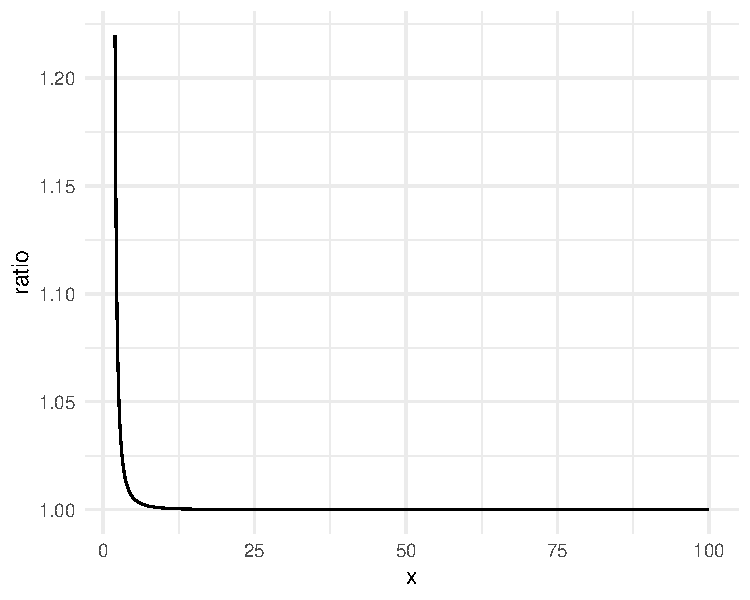
\includegraphics{Homework1_files/figure-latex/exe_1.14b-1} \end{center}

\hypertarget{exercise-1.15}{%
\subsubsection{Exercise 1.15}\label{exercise-1.15}}

The second derivative of the log-gamma function is called the trigamma
function: \[\Psi ' (x) = \frac{d^2}{dx^2}\log\Gamma(x).\] Like the
digamma function, it often arises in statistical calculations; for
example, see Exercise 1.35.

\begin{enumerate}
\def\labelenumi{\alph{enumi}.}
\tightlist
\item
  Using the method of Exercise 1.13(c) with \(h = 1\) {[}that is,
  expanding \(f(x+2h), f(x+h), f(x-h),\) and \(f(x-2h)\) and then
  finding a linear combination that makes all but the \textit{second}
  derivative of the log-gamma function disappear{]}, show how to derive
  the following approximation to \(\Psi ' (x)\) for \(x>2:\)
  \[\Psi '(x) \approx \frac{1}{12}\log\left[\left(\frac{x}{x-1}\right)^{15}\left(\frac{x-2}{x+1}\right)\right]\]
\end{enumerate}

Let \(f(x) = \log\Gamma(x).\) Then
\(f'(x) = \Psi(x) = \frac{d}{dx}\log\Gamma(x)\) and
\(f''(x) = \Psi'(x) = \frac{d^2}{dx^2}\log\Gamma(x).\) Using Taylor
Series to expand:

\begin{align*}
f(x+1) & \approx f(x) + f'(x) + \frac{1}{2} f''(x) + \frac{1}{6}f'''(x) + \frac{1}{24}f''''(x)\\
f(x) & \approx f(x)\\
f(x-1) & \approx f(x) - f'(x) + \frac{1}{2} f''(x) - \frac{1}{6}f'''(x) + \frac{1}{24}f''''(x)\\
\\
f(x+2) & \approx f(x) + f'(x) + 2f''(x) + \frac{8}{6}f'''(x) + \frac{16}{24}f''''(x)\\
f(x) & \approx f(x)\\
f(x-2) & \approx f(x) - f'(x) + 2f''(x) - \frac{8}{6}f'''(x) + \frac{16}{24}f''''(x)\\
\end{align*}

Then, \(f(x+1)-2f(x)+f(x-1) = f''(x)+\frac{1}{12}f''''(x)\) and
\(f(x+2)-2f(x)+f(x-2) = 4f''(x)+\frac{16}{12}f''''(x)\). Therefore,
\[f''(x) \approx \frac{16[f(x+1)-2f(x)+f(x-1)]-[f(x+2)-2f(x)+f(x-2)]}{12}.\]
Then using equation 1.15, \begin{align*}
\Gamma(x+1)&=x\Gamma(x)\\
\Gamma(x+2)&=(x+1)x\Gamma(x)\\
\Gamma(x-1)&=\frac{\Gamma(x)}{x-1}\\
\Gamma(x-2)&=\frac{\Gamma(x)}{(x-1)(x-2)}.
\end{align*}

Thus, plugging in \(f(x) = \log\Gamma(x)\) and using the above
identities, we obtain,
\[\Psi'(x)\approx \frac{1}{12}\log\left(\left(\frac{x}{x-1}\right)^{15}\left(\frac{x-2}{x+1}\right)\right).\]

\begin{enumerate}
\def\labelenumi{\alph{enumi}.}
\setcounter{enumi}{1}
\tightlist
\item
  Test Approximation 1.18 numerically as in Exercise 1.14(b). In R or
  Splus, \texttt{trigamma(x)} gives the value of \(\Psi ' (x)\)
\end{enumerate}

Similar to 1.14(b), the approximation does not appear to perform well
for \(x\) close to 2. However, the approximation performs better for
larger values of \(x\).

\begin{Shaded}
\begin{Highlighting}[]
\NormalTok{x <-}\StringTok{ }\KeywordTok{seq}\NormalTok{(}\DataTypeTok{from =} \DecValTok{2}\NormalTok{, }\DataTypeTok{to =} \DecValTok{100}\NormalTok{, }\DataTypeTok{by =} \FloatTok{0.01}\NormalTok{)}
\NormalTok{ratio <-}\StringTok{ }\DecValTok{12} \OperatorTok{*}\StringTok{ }\KeywordTok{trigamma}\NormalTok{(x)}\OperatorTok{/}\KeywordTok{log}\NormalTok{((x}\OperatorTok{/}\NormalTok{(x }\OperatorTok{-}\StringTok{ }\DecValTok{1}\NormalTok{))}\OperatorTok{^}\NormalTok{\{}
    \DecValTok{15}
\NormalTok{\} }\OperatorTok{*}\StringTok{ }\NormalTok{((x }\OperatorTok{-}\StringTok{ }\DecValTok{2}\NormalTok{)}\OperatorTok{/}\NormalTok{(x }\OperatorTok{+}\StringTok{ }\DecValTok{1}\NormalTok{)))}
\NormalTok{data_}\FloatTok{1.15}\NormalTok{b <-}\StringTok{ }\KeywordTok{as.data.frame}\NormalTok{(}\KeywordTok{cbind}\NormalTok{(x, ratio))}
\KeywordTok{library}\NormalTok{(ggplot2)}
\KeywordTok{ggplot}\NormalTok{(}\DataTypeTok{data =}\NormalTok{ data_}\FloatTok{1.15}\NormalTok{b, }\KeywordTok{aes}\NormalTok{(}\DataTypeTok{x =}\NormalTok{ x, }\DataTypeTok{y =}\NormalTok{ ratio)) }\OperatorTok{+}\StringTok{ }
\StringTok{    }\KeywordTok{geom_line}\NormalTok{() }\OperatorTok{+}\StringTok{ }\KeywordTok{theme_minimal}\NormalTok{()}
\end{Highlighting}
\end{Shaded}

\begin{center}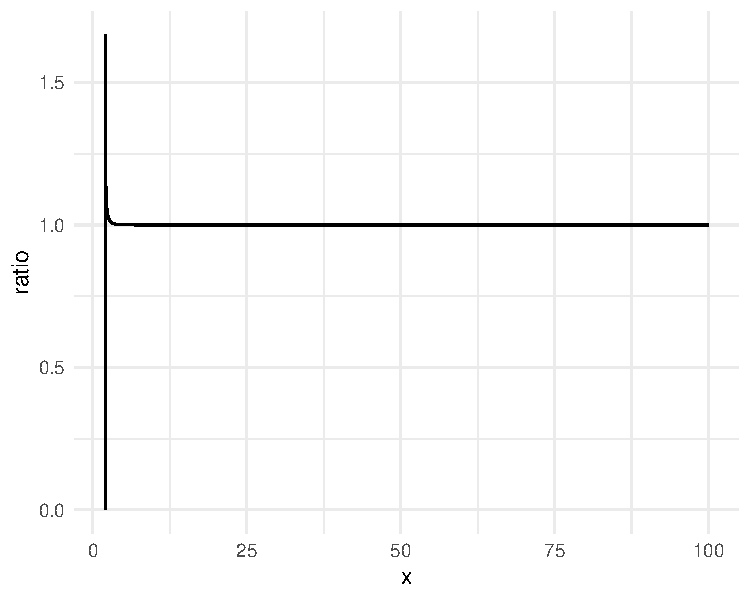
\includegraphics{Homework1_files/figure-latex/exe_1.15b-1} \end{center}

\hypertarget{exercise-1.18}{%
\subsubsection{Exercise 1.18}\label{exercise-1.18}}

Suppose that \(a_n \sim b_n\) and \(c_n \sim d_n\).

\begin{enumerate}
\def\labelenumi{\alph{enumi}.}
\tightlist
\item
  Prove that \(a_nc_n \sim b_nd_n.\)
\end{enumerate}

\begin{proof}
Since $a_n \sim b_n$ and $c_n \sim d_n$, then $a_n/b_n \rightarrow 1$ and $c_n/d_n \rightarrow 1$. Then $$\frac{a_nc_n}{b_nd_n} = \frac{a_n/b_n}{c_n/d_n}\rightarrow \frac{1}{1} = 1.$$ Therefore, $a_nc_n \sim b_nd_n.$
\end{proof}

\begin{enumerate}
\def\labelenumi{\alph{enumi}.}
\setcounter{enumi}{1}
\tightlist
\item
  Show by counterexample that it is not generally true that
  \(a_n + c_n \sim b_n + d_n.\)
\end{enumerate}

Let \(a_n = n, b_n = n + 1, c_n = -n,\) and \(d_n = -n.\) Then
\(\frac{a_n}{b_n} = \frac{n}{n+1} \rightarrow 1\) and
\(\frac{c_n}{d_n} = \frac{-n}{-n} \rightarrow 1.\) Therefore,
\(a_n \sim b_n\) and \(c_n \sim d_n\). However,
\[\frac{a_n + c_n}{b_n + d_n}=\frac{n-n}{n+1-n} = 0/1 \rightarrow 0.\]
Thus, \(a_n + c_n \sim b_n + d_n\) does not hold.

\begin{enumerate}
\def\labelenumi{\alph{enumi}.}
\setcounter{enumi}{2}
\tightlist
\item
  Prove that \(|a_n| + |c_n| \sim |b_n| + |d_n|.\)
\end{enumerate}

\begin{proof}
Since $a_n \sim b_n$ and $c_n \sim d_n$, $\left|\frac{a_n-b_n}{a_n}\right|\rightarrow 0$ and $\left|\frac{c_n-d_n}{c_n}\right|\rightarrow 0$. Then

\begin{align*}
\left|\frac{(|a_n|+|c_n|)-(|b_n|+|d_n|)}{|a_n|+|c_n|}\right| & = \left|\frac{(|a_n|-|b_n|)+(|c_n|-|d_n|)}{|a_n|+|c_n|}\right|\\
& = \left|\left(\frac{|a_n|}{|a_n|+|c_n|}\right)\left(\frac{|a_n|-|b_n|}{|a_n|}\right)+\left(\frac{|c_n|}{|a_n|+|c_n|}\right)\left(\frac{|c_n|-|d_n|}{|c_n|}\right)\right|\\
& \rightarrow C_1\cdot 0 + C_2 \cdot 0\\
& = 0.
\end{align*}

Thus, since $$\left|\frac{(|a_n|+|c_n|)-(|b_n|+|d_n|)}{|a_n|+|c_n|}\right|\rightarrow 0,$$
$|a_n| + |c_n| \sim |b_n| + |d_n|.$
\end{proof}

\begin{enumerate}
\def\labelenumi{\alph{enumi}.}
\setcounter{enumi}{3}
\tightlist
\item
  Show by counterexample that it is not generally true that
  \(f(a_n) \sim f(b_n)\) for a continuous function \(f(x)\).
\end{enumerate}

Let \(a_n = n^2+n\) and \(b_n = n^2\). Consider \(f(x) = e^x.\) Then
\(\frac{a_n}{b_n} = \frac{n^2+n}{n^2}\rightarrow 1\), but
\(\frac{e^{n^2+n}}{e^{n^2}} = e^x \rightarrow \infty.\) Therefore,
\(f(a_n) \sim f(b_n)\) does not hold.


\end{document}
